A core aspect of human intelligence is adapting to new tasks quickly while drawing upon relevant past learning experiences. Meta-learning  ~\citep{schmidhuber1987, thrun2012learning, Naik1992MetaneuralNT} can achieve this by identifying common structures among various tasks, which enables faster learning of a new task with as little data as possible. Recent works ~\citep{santoro2016meta, vinyals2016matching, finn2017model} show that meta-learning algorithms can learn new tasks with as little as one example. 
However, existing meta-learning techniques (\emph{e.g.,} MAML) often fail to generalize well when the test tasks belong to a different distribution from the training tasks distribution~\citep{Chen2019ICLR}. For example, MAML assumes equal weights to all samples in the same task and equal weights to all tasks in the training task distribution during expected meta-training loss minimization. This task homogeneity assumption of MAML often limits its ability to work in real-world applications. 

%However, existing meta-learning techniques (\emph{e.g.,} MAML) often fail to generalize well when the test tasks belong to a different distribution from the training tasks distribution~\citep{Chen2019ICLR}.  For example, MAML assumes equal weightage to all samples in the same task and equal weightage to all tasks in the training task distribution during expected meta-training loss minimization. Hence, it assumes that meta-train distribution is the same as meta-test distribution—this assumption of no domain shift is severely unrealistic, severely limiting its capability in real-world applications.
%A core aspect of human intelligence is adapting to new tasks quickly while drawing upon relevant past learning experiences. Similarly, meta-learning algorithms try to adapt to a new task using a smaller number of examples. Past work ~\citep{schmidhuber1987, thrun2012learning, Naik1992MetaneuralNT} has shown that meta-learning algorithms can achieve this by identifying common structures among various tasks, which in turn enables faster learning of a new task with as little data as possible. Recent works ~\cite{santoro2016meta, vinyals2016matching, finn2017model} shows that meta-learning algorithms can learn new tasks with as little as one example. One particular algorithm that has shown great success over the past few years is the model-agnostic meta-learning (MAML) framework~\citep{finn2017model}. 

\begin{figure}[!t]
%\captionsetup[subfigure]{aboveskip=-2pt,belowskip=-2pt}
    \centering
    \includegraphics[width=0.48\textwidth, height=4cm]{Robust Meta Learning/figs/motivation.png}
    \caption{Types of Domain Shift. Solid green squares and circles represent tasks sampled from the in-distribution dataset (\textit{e.g.,} \textit{mini}-ImageNet~\citep{ravi2016optimization}); red triangles indicate tasks sampled from out-of-distribution (OOD) dataset (\textit{e.g.,} SVHN~\citep{netzer2011reading}). Training and testing domains (a) are subsets of the data domain; (b) have some overlap between each other where some OOD tasks (\textit{e.g.} $30\%$, etc.) are involved in the training domain; \textbf{We consider type (b), partial domain shift, in our paper}.}
    \label{fig:motivation}
\vspace{-5mm}
\end{figure}

\begin{figure*}[!htbp]
%\captionsetup[subfigure]{aboveskip=-2pt,belowskip=-2pt}
    \centering
    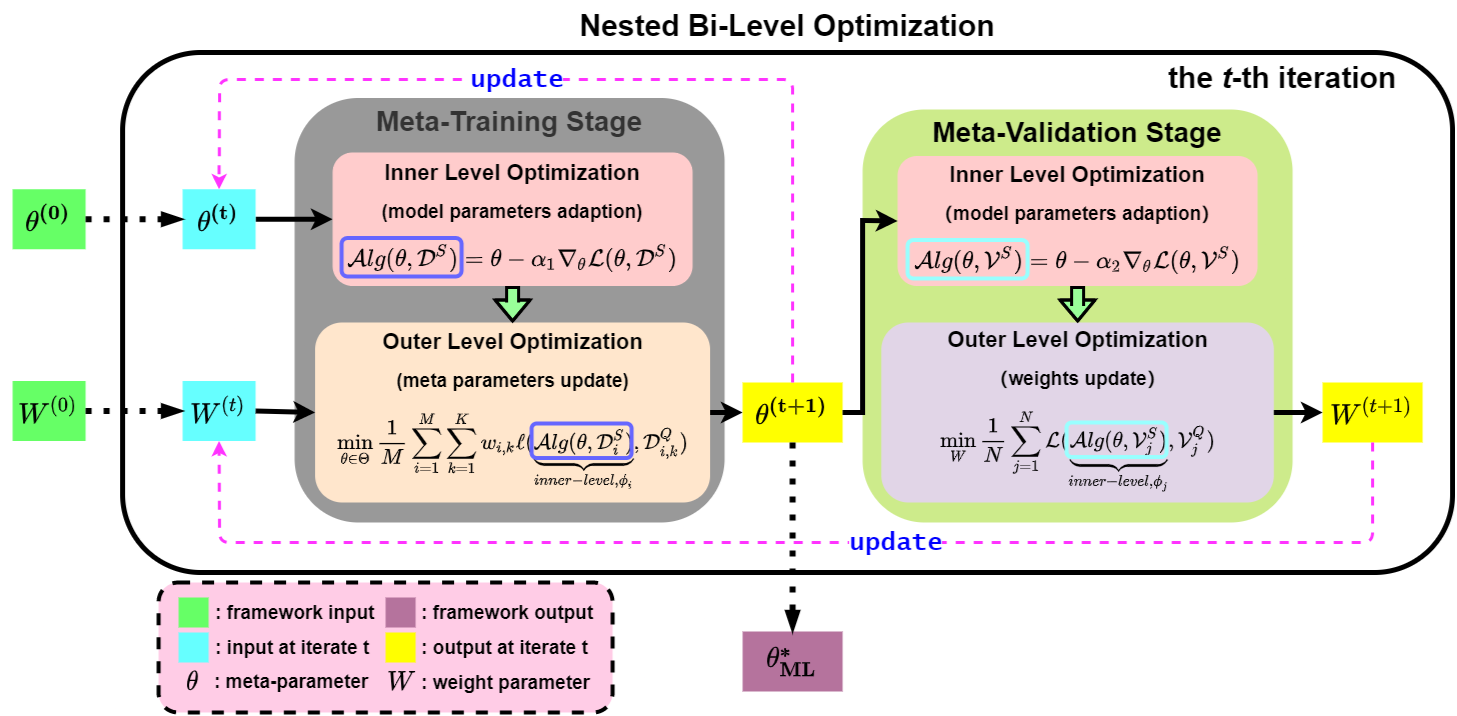
\includegraphics[width=0.8\linewidth, height=6.5cm]{Robust Meta Learning/figs/overview.png}
    \caption{Overview of our \sysname{} framework that solves a \biopt{} optimization problem. (a) In the meta-training stage, model parameters $\phi_i$ of each task are adapted from meta-parameter $\boldsymbol{\theta}$ through the inner level optimization; (b) In the outer-level of the meta-training stage, we update the meta-parameters using the weights $W$ from the previous iterate; (c) Weights are further updated in the meta-validation stage using the gradient of the meta-losses with respect to current $W$.} 
    \label{fig:overview}
    \vspace{-5mm}
\end{figure*}

%However, existing meta-learning techniques (\emph{e.g.,} MAML) often fail to generalize well when the test tasks belong to a different distribution from the training tasks distribution~\citep{Chen2019ICLR}. For example, MAML assumes equal weightage to all samples in the same task and equal weightage to all tasks in the training task distribution during expected meta-training loss minimization. Hence, it assumes that meta-train distribution is the same as meta-test distribution—this assumption of no domain shift is severely unrealistic, severely limiting MAML's knowledge transfer capability in real-world applications. Figure \ref{fig:motivation} illustrates three situations regarding domain shifts between the meta-training and meta-testing stages (i.e., same task distributions, overlap in task distributions, no overlap in task distributions) that can occur in real-world scenarios.

% MAML tries to identify optimal initial parameters of the model that minimize the expected loss on the whole task distribution after one or a few gradient steps. MAML assumes equal weights to all samples in the same task and equal weights to all the tasks in the training task distribution while calculating the expected loss. This assumption is limited to real-world applications and hence current few-shot classification algorithms fail to address the problem in which the meta-training domain is shifted from meta-testing domain~\citep{Chen2019ICLR}. Figure \ref{fig:motivation} illustrates three situations regarding domain shifts between the meta-training and meta-testing stages. Existing meta-learning techniques (\textit{e.g.} MAML), focuses on recognizing novel class with limited training examples. These novel classes, however, are sampled from the same data domain. As for knowledge transfer, the lack of domain shift makes the evaluation scenarios unrealistic. To this end, in this paper we address the problem by introducing out-of-distribution (OOD) tasks which are sampled different from data distribution \textcolor{red}{...}
% \subsection{Motivating Applications}
% A meta-learner~\citep{thrun2012learning} seeks to find universal properties among all the relevant tasks learned, which reduces the model hypothesis's search space for optimal model parameters. In contrast, 

\vspace{-1ex}
\subsection{Motivation} 
{\color{red} add one paragraph to discuss the SOTA methods to the introduction to explain the motivation
2. connection to traditional robust model, generalize the l2rw and metawtNet from instance level to task level in FSL. Traditional methods..., the goal of ours is to learn a ...}
We illustrate the presence of domain shift in the real-world application through a series of examples. The first example is detecting vehicles at night, where the meta-test tasks consist of images of vehicles at night, whereas meta-training tasks consist of images of the vehicles in multiple lighting scenarios.  Another example is rare lung cancer detection, where the meta-test tasks contain images belonging to rare lung cancer, whereas meta-training tasks consist of general cancer x-ray images.  In both the examples given above, meta-test tasks belong to specialized slices where the data availability is meager compared to meta-training tasks. Hence, it is essential to consider the meta-test data distribution during the meta-training stage to leverage meta-learning in such scenarios. Figure \ref{fig:motivation} illustrates three situations regarding domain shift between the meta-training and meta-testing task sets that can occur in real-world scenarios. In this work, we focus on type (b) distribution shift, where the meta-training has tasks which are out of distribution to the meta-training tasks (i.e. the meta-test dataset is a specialized slice of meta-train). Another problem which occurs in real world few shot learning problems is that some of the labels might be noisy (either due to human errors in labeling or inherent ambiguity of certain classification problems). A natural way of dealing with out-of-distribution (OOD) tasks or noisy labeled data in meta-training is by assigning weights to either tasks or individual instances. For example, assigning a weight of zero to OOD or noisy tasks/instances in the meta-train set improves the meta-learning algorithm's performance. The resulting problem is an extension of meta-learning called \emph{weighted meta-learning}. Weighted meta-learning has been studied in~\citep{cai2020weightedmeta}, where they study the weighting on a restricted class of loss functions like the square loss and hinge loss. In contrast, in this work, we propose a framework called \sysname{} that can {\textit{a}}) handle arbitrary loss functions and \textit{b}) jointly learn the weights along with the meta-learning model parameters. 
%An efficient meta-learning algorithm should learn the corresponding meta-knowledge of vehicle detection or tumor detection useful for faster learning of specialized tasks like detecting vehicles at night or rare cancer.

\vspace{-1ex}
\subsection{Our Contributions}
Our work's significant contribution is introducing the nested MAML (\sysname{}) algorithm, an end-to-end framework for the reweighted MAML training. \sysname{} considers the weights as hyper-parameters and uses a small set of meta-validation tasks representing the meta-test tasks to find the optimal hyper-parameters by minimizing the meta-loss on the validation tasks in a \textbf{\biopt{}} manner.  An overview of \sysname{} is given in Figure \ref{fig:overview}. In practice, the size of the meta-validation tasks set required by \sysname{} is tiny compared to the meta-training dataset. Hence, it is neither expensive nor unrealistic to create a  small and clean meta-validation set even for rare specialized use cases of a real-life scenario. A similar strategy has been applied in ~\citep{ren2018learning,shu2019meta,killamsetty2020glister}. However, they focus on traditional supervised learning, and we apply this in a meta-learning setting. Since \sysname{} uses an online framework to perform a joint optimization of the weight hyper-parameters and model parameters for the weighted MAML model, the computational time of \sysname{} is comparable to MAML.
% specifically 1.5 times MAML's running time. %Finally, we compare \sysname{}'s performance to existing robust meta-learning and hyperparameter optimization algorithms through extensive experiments on real-world and synthetic datasets for {\textcolor{red}{out-of-distribution (OOD), noisy-labels settings in training data}}.

\noindent \textbf{Contributions of our work are summarized as follows:} 
%1) We study the general form of the instance and task weighted meta learning, where we learn the optimal weights by optimizing a \textit{\biopt{}} objective function. To the best of our knowledge, ours is the first work that studies the \textit{\biopt{}} optimization problem, which comes naturally in such a setting, 2)We introduce a novel algorithmic framework \sysname{} that uses a small set of validation tasks to enable robust meta-learning. We solve the \emph{\biopt{}} optimization problem efficiently through a series of practical approximations and provide a theoretical convergence analysis for \sysname{}. In particular, we show that \sysname{} converges in $\mathcal{O}(1/\epsilon^2)$ iterations under reasonable assumptions, and contrast this with existing bounds of MAML, and 3)We provide comprehensive synthetic and real-world data experiments demonstrating that \sysname{} achieves state-of-the-art results in two scenarios (OOD tasks and noisy labels).
%\vspace{-1ex}
%\begin{itemize}[leftmargin=*]
1) We study the general form of the instance and task weighted meta learning, where we learn the optimal weights by optimizing a \textit{\biopt{}} objective function. To the best of our knowledge, ours is the first work that studies the \textit{\biopt{}} optimization problem, which comes naturally in such a setting. 2) We introduce a novel algorithmic framework \sysname{} that uses a small set of validation tasks to enable robust meta-learning. We solve the \emph{\biopt{}} optimization problem efficiently through a series of practical approximations and provide a theoretical convergence analysis for \sysname{}. In particular, we show that \sysname{} converges in $\mathcal{O}(1/\epsilon^2)$ iterations under reasonable assumptions, and contrast this with existing bounds of MAML. 3) We provide comprehensive synthetic and real-world data experiments demonstrating that \sysname{} achieves state-of-the-art results in two scenarios (OOD tasks and noisy labels).
%\end{itemize}

\vspace{-1ex}
\subsection{Related Work}
\textbf{Meta Learning.} There are several lines of meta-learning algorithms for base learners: nearest neighbors-based methods ~\citep{vinyals2016matching, snell2017prototypical}, recurrent network-based methods ~\citep{ravi2016optimization}, and gradient-based methods. As the representative of a gradient-based meta-learning algorithm, MAML~\citep{finn2017model} and its variants ~\citep{finn2018probabilistic, antoniou2018train, nichol2018first, rusu2018meta,rajeswaran2019meta, behl2019alpha, raghu2019rapid, zhao2020fair} learn a shared initialization of model parameters across a variety of tasks during the meta-training phase that can adapt to new tasks using a few gradient steps. ~\citeauthor{cai2020weightedmeta} proposes a simple weighted meta-learning approach for the basis regression problem that selects weights by minimizing a data-dependent bound involving an empirical integral probability metric between the weighted sources and target risks. However, this approach cannot be easily extended to complex scenarios with arbitrary loss functions. % Our \sysname{} algorithm poses the weights as hyper-parameters of the model and tries to estimate these weights by minimizing the nested loss over the model parameters and weight hyper-parameters. \sysname{} can be applied to any loss functions at the expense of the computational costs due to the need for higher-order differentiation in the computation graph.
% ~\cite{yao2020automated} proposes ARML, which extracts the cross-task relations and constructs the meta-knowledge graph to enable the model to find a specific meta learner for the new task.

\textbf{Learning with OOD tasks.} %Because of task homogeneity assumption limitation, MAML does not perform well on the training tasks sampled from different distributions ~\citep{vuorio2019multimodal}. 
Several robust meta-learning approaches ~\citep{vuorio2019multimodal, triantafillou2019meta,yao2020automated} were proposed to deal with OOD tasks in meta-training tasks set. Using a probabilistic meta-learning perspective, {\color{red}~\cite{lee2020l2b} proposes a Bayesian inference framework and variational inference to deal with OOD tasks.} Similar to our OOD tasks setting, ~\cite{vuorio2019multimodal} proposed  MMAML to deal with multimodal task distribution with disjoint and far apart modes and proposes a model that generates a set of separate meta-learned prior parameters to deal with each mode of a multimodal distribution. ({\color{red} explain the baselines more clear})
%Among the meta-training tasks, some tasks are Out-of-Distribution (OOD) if they have a very different distribution from others. 

\textbf{Learning with noisy labels.} Samples with corrupted labels are ubiquitous in real-world datasets. Several methods ~\citep{luo2015foveation, jalal2017robust, wang2019direct} discuss noise-robust models to tackle noisy samples.~\citet{ren2018learning, shu2019meta} propose a noisy data filtering strategy using an instance reweighting strategy where the weights are learned automatically. However, the effect of noisy labels on few-shot learning requires more attention. Although ~\cite{lu2020robust} proposes robust few-shot learning, they assume a presence of a biased meta episode that contains synthesized information of outlier and noisy samples. In contrast, \sysname{} does not require any additional information about noisy samples in its learning.%to deal with the training tasks containing data instances with noisy labels. 

% In contrast, ~\citep{han2018co, chen2019understanding}propose noisy data filtering techniques to reduce noisy labels' impact. 
%Our paper is the first to consider the training tasks with noisy labels without any additional information about noisy samples in the few-shot learning framework to the best of our knowledge. 

%for noise filtering that solves a bi-level optimization problem on instance weights. In contrast~\cite{shu2019meta} uses an MLP as a weighting function, explicitly mapping sample weights adaptively from the data. 
%Many researchers focus on learning with noisy labels to avoid extravagant relabeling costs by improving deep learning models' robustness.
% ~\cite{han2018co} proposes a co-teaching model that trains two neural networks simultaneously, and they will teach each other to detect noisy samples. INCV~\citep{chen2019understanding} applies cross-validation to randomly split noisy datasets and use the selected samples to train the model. ~\cite{ren2018learning} proposes a gradient-based method to assign weights to training samples by online meta-learning strategy.
% For comparison, we consider two baselines that use Co-teaching~\citep{han2018co} and INCV~\citep{chen2019understanding} to clean noisy datasets first and apply MAML to the selected data.